\section{Experimentos}
\label{sec:experimentos}
	A continuacion como resultado se muestran algunas imagenes de partidas jugadas contra la propia heuristica, el jugador ninja y un jugador humano. Los tres `Jugadores'  citados anteriormente juegan con las fichas azules, es decir cada vez que se ve el mensaje `GANA EL JUGADOR VERDE' es la IA programada en esta practica la que vence.


	Partida en la que se ha probado la heuristica 1 programada jugando contra ella misma:

		\begin{figure} [H]
			\begin{center}
				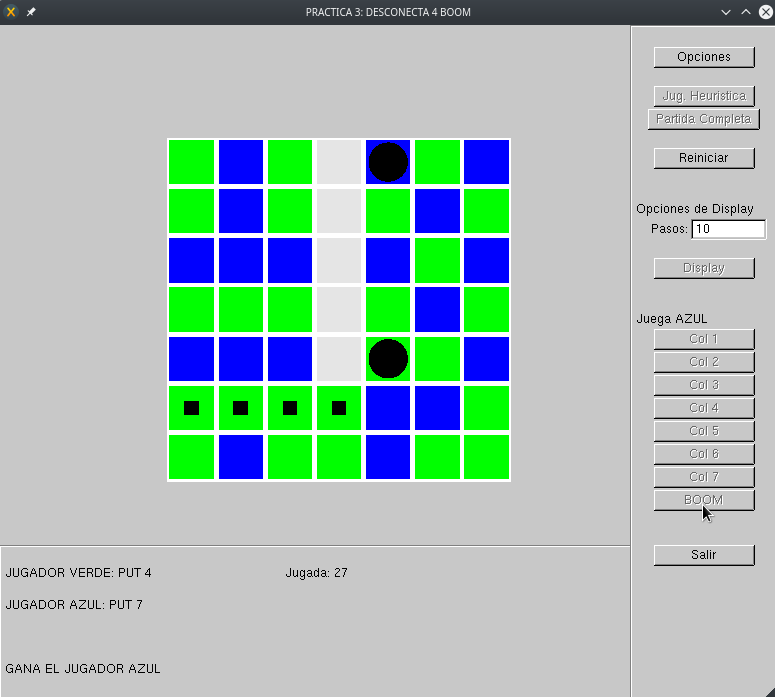
\includegraphics[width=9cm]{HeurVSHeur}
				\caption{Captura de la partida Heur Vs Heur}
				\label{uno}
			\end{center}
		\end{figure}

 	A continuación se muestra una partida contra el jugador ninja que se supone tiene buena heuristica implementada:

 	\begin{figure}[H]
 		\begin{center}
		 	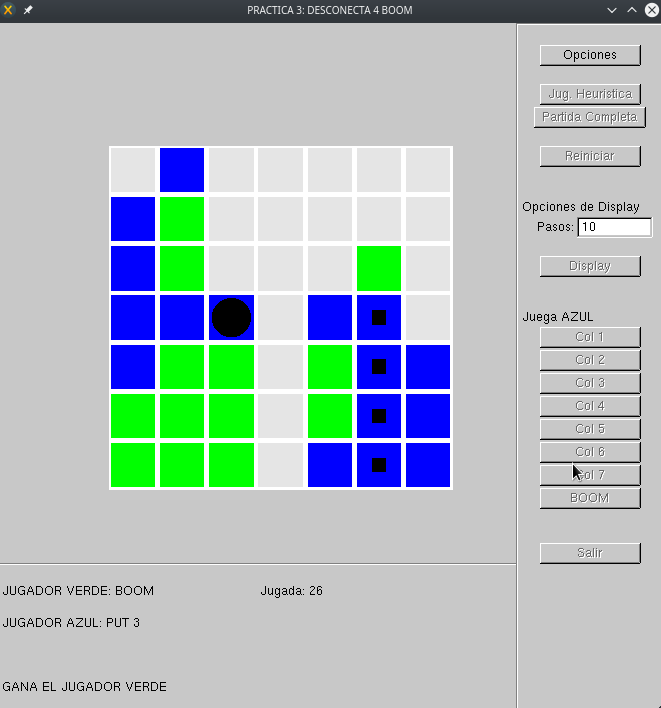
\includegraphics[width=9cm]{HeurVSNinja.png}
		 	\caption{Captura de la partida Heuristica VS Ninja}
		 	\label{dos}
 		\end{center}
 	\end{figure}


 	Y una partida contra el jugador ninja en la que la IA es el  jugador 2 (AZUL).

 	\begin{figure}[H]
		\begin{center}
	 	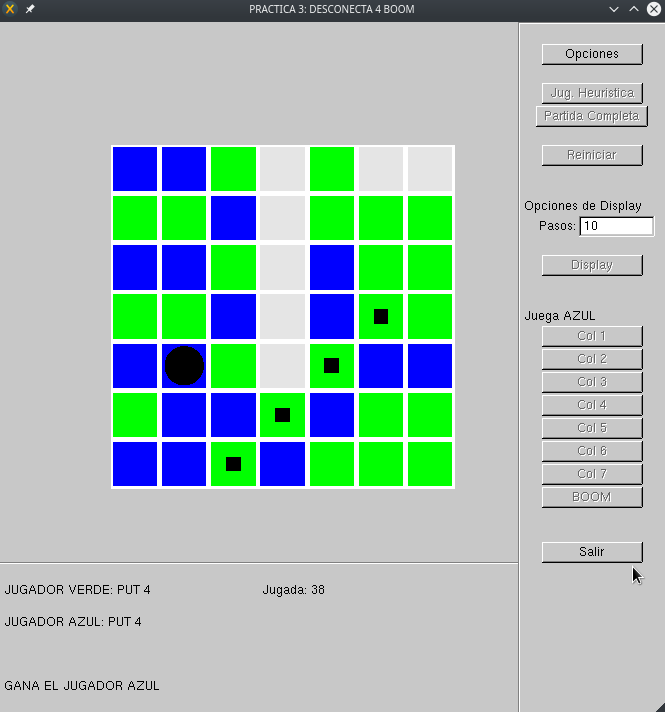
\includegraphics[width=9cm]{NinjaVSHeur.png}
	 	\caption{Captura de la partida Heuristica VS Ninja}
	 	\label{dos}
		\end{center}
	\end{figure}

	Con la segunda heuristica se ha obtenido un 100\% de exito en las partidas contra el jugador ninja.

 %	Partida jugada contra un jugador humano:

% 	\begin{figure}[H]
%	 	\includegraphics[width=10cm]{HeurVSHuman}
%	 	\caption{Captura de la partida Heuristica VS Humano}
%	 	\label{tres} 
% 	\end{figure}


